% !TEX TS-program = pdflatex
% !TEX encoding = UTF-8 Unicode

% This is a simple template for a LaTeX document using the "article" class.
% See "book", "report", "letter" for other types of document.

\documentclass[11pt]{article} % use larger type; default would be 10pt

\usepackage[utf8]{inputenc} % set input encoding (not needed with XeLaTeX)
\usepackage[spanish]{babel}

%%% Examples of Article customizations
% These packages are optional, depending whether you want the features they provide.
% See the LaTeX Companion or other references for full information.

%%% PAGE DIMENSIONS
\usepackage{geometry} % to change the page dimensions
\geometry{a4paper} % or letterpaper (US) or a5paper or....
% \geometry{margin=2in} % for example, change the margins to 2 inches all round
% \geometry{landscape} % set up the page for landscape
%   read geometry.pdf for detailed page layout information

\usepackage{graphicx} % support the \includegraphics command and options
\usepackage[outdir=./]{epstopdf}
% \usepackage[parfill]{parskip} % Activate to begin paragraphs with an empty line rather than an indent
\usepackage{listings}

%%% PACKAGES
\usepackage{booktabs} % for much better looking tables
\usepackage{array} % for better arrays (eg matrices) in maths
\usepackage{paralist} % very flexible & customisable lists (eg. enumerate/itemize, etc.)
\usepackage{verbatim} % adds environment for commenting out blocks of text & for better verbatim
%\usepackage{subfig} % make it possible to include more than one captioned figure/table in a single float
\usepackage{subcaption}
\usepackage{url}
\usepackage{diagbox}
\usepackage{amsmath}
\usepackage{pdfpages}
% These packages are all incorporated in the memoir class to one degree or another...
%\usepackage[hidelinks]{hyperref}
\usepackage{hyperref}

\usepackage{xcolor}
\hypersetup{
    colorlinks,
    linkcolor={red!50!black},
    citecolor={blue!50!black},
    urlcolor={blue!80!black}
}

%%% HEADERS & FOOTERS
\usepackage{fancyhdr} % This should be set AFTER setting up the page geometry
\pagestyle{fancy} % options: empty , plain , fancy
\renewcommand{\headrulewidth}{0pt} % customise the layout...
\lhead{}\chead{}\rhead{}
\lfoot{}\cfoot{\thepage}\rfoot{}

%%% SECTION TITLE APPEARANCE
\usepackage{sectsty}
\allsectionsfont{\sffamily\mdseries\upshape} % (See the fntguide.pdf for font help)
% (This matches ConTeXt defaults)

%%% ToC (table of contents) APPEARANCE
\usepackage[nottoc,notlof,notlot]{tocbibind} % Put the bibliography in the ToC
\usepackage[titles,subfigure]{tocloft} % Alter the style of the Table of Contents
\renewcommand{\cftsecfont}{\rmfamily\mdseries\upshape}
\renewcommand{\cftsecpagefont}{\rmfamily\mdseries\upshape} % No bold!

%%% END Article customizations

%%% The "real" document content comes below...

\title{CLP Lab 7 Report}
\author{Albert Aparicio Isarn\\
        \href{mailto:albert.aparicio.isarn@alu-etsetb.upc.edu}{\nolinkurl{albert.aparicio.isarn@alu-etsetb.upc.edu} }
	\and
	Héctor Esteban Cabezos\\
        \href{mailto:hect.esteban@gmail.com}{\nolinkurl{hect.esteban@gmail.com}}}
\date{} % Activate to display a given date or no date (if empty),
         % otherwise the current date is printed

\begin{document}

	% ---- MATLAB Code definitions ----- %
	\definecolor{mygreen}{rgb}{0,0.6,0}
	\definecolor{mygray}{rgb}{0.5,0.5,0.5}
	\definecolor{mymauve}{rgb}{0.58,0,0.82}

	\lstset{ %
		%backgroundcolor=\color{white},   % choose the background color; you must add \usepackage{color} or \usepackage{xcolor}
		basicstyle=\ttfamily\footnotesize,        % the size of the fonts that are used for the code
		breakatwhitespace=false,         % sets if automatic breaks should only happen at whitespace
		breaklines=true,                 % sets automatic line breaking
		captionpos=b,                    % sets the caption-position to bottom
		commentstyle=\color{mygreen},    % comment style
		deletekeywords={...},            % if you want to delete keywords from the given language
		escapeinside={\%*}{*)},          % if you want to add LaTeX within your code
		extendedchars=true,              % lets you use non-ASCII characters; for 8-bits encodings only, does not work with UTF-8
		%frame=single,	                   % adds a frame around the code
		keepspaces=true,                 % keeps spaces in text, useful for keeping indentation of code (possibly needs columns=flexible)
		keywordstyle=\color{blue},       % keyword style
		language=Matlab,                 % the language of the code
		otherkeywords={*,...},            % if you want to add more keywords to the set
		%numbers=left,                    % where to put the line-numbers; possible values are (none, left, right)
		%numbersep=5pt,                   % how far the line-numbers are from the code
		%numberstyle=\tiny\color{mygray}, % the style that is used for the line-numbers
		rulecolor=\color{black},         % if not set, the frame-color may be changed on line-breaks within not-black text (e.g. comments (green here))
		showspaces=false,                % show spaces everywhere adding particular underscores; it overrides 'showstringspaces'
		showstringspaces=false,          % underline spaces within strings only
		showtabs=false,                  % show tabs within strings adding particular underscores
		stepnumber=2,                    % the step between two line-numbers. If it's 1, each line will be numbered
		stringstyle=\color{mymauve},     % string literal style
		tabsize=2,	                   % sets default tabsize to 2 spaces
		title=\lstname                   % show the filename of files included with \lstinputlisting; also try caption instead of title
	}

\maketitle

\section{Programación de método de clasificación}

El script \textbf{\texttt{main\_2\_1}} contiene el código del ejercicio 1. En
la sección \ref{src:main:21} se puede ver su código fuente.

La sección 2 de este ejercicio corresponde a la función
\textbf{\texttt{CLP\_Kmeans}}, cuyo código fuente se muestra en la sección
\ref{src:fun:kmeans}.

A continuación se muestran los resultados de este ejercicio. En la figura
\ref{fig:21:clusters} se muestra la base de datos creada
por \textbf{\texttt{CLP\_Generate}} (código fuente en la sección
\ref{src:fun:generate}) y el resultado de la clasificación con 4, 9 y 10
\emph{clusters}.

Esta función genera los \emph{clusters} con parámetros (media y varianza)
aleatorios, al igual que las probabilidades a priori de los $L$ \emph{clusters}.

En los resultados de la clasificación de la figura \ref{fig:21:clusters} se
pueden ver también algunas de las evoluciones de los centroides. No se ven todas
porque algunos centroides quedan ''ocultos'' dentro de la nube de puntos del
\emph{cluster}.

\begin{figure}%[h]
    \centering
    \begin{subfigure}[b]{0.3\textwidth}
        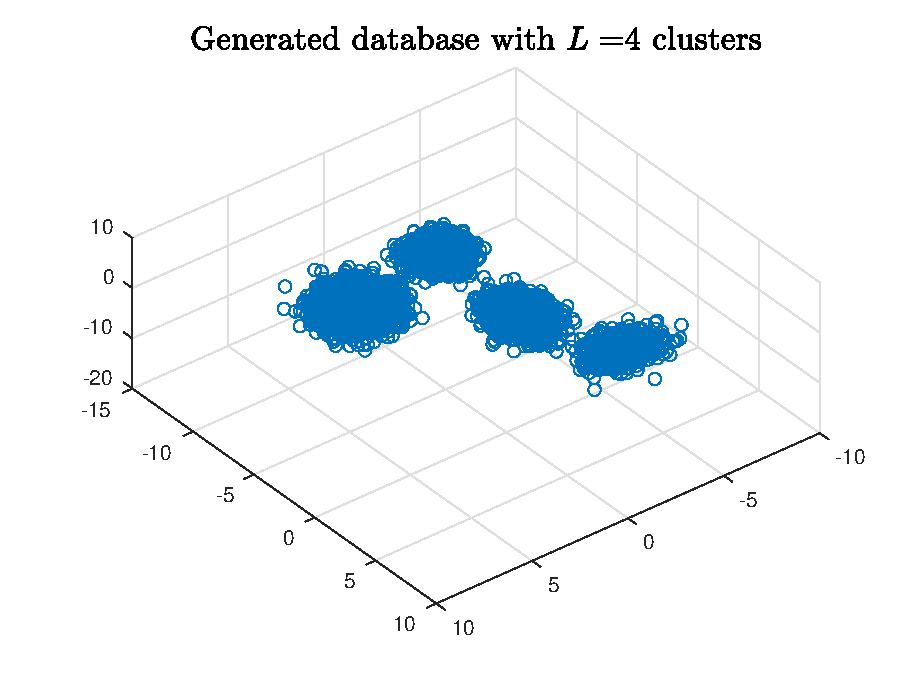
\includegraphics[width=\textwidth]{../src/fig/21_database.eps}
        \caption[]{Base de datos sintética}
        \label{fig:21:db}
    \end{subfigure}
    \quad
    \begin{subfigure}[b]{0.3\textwidth}
        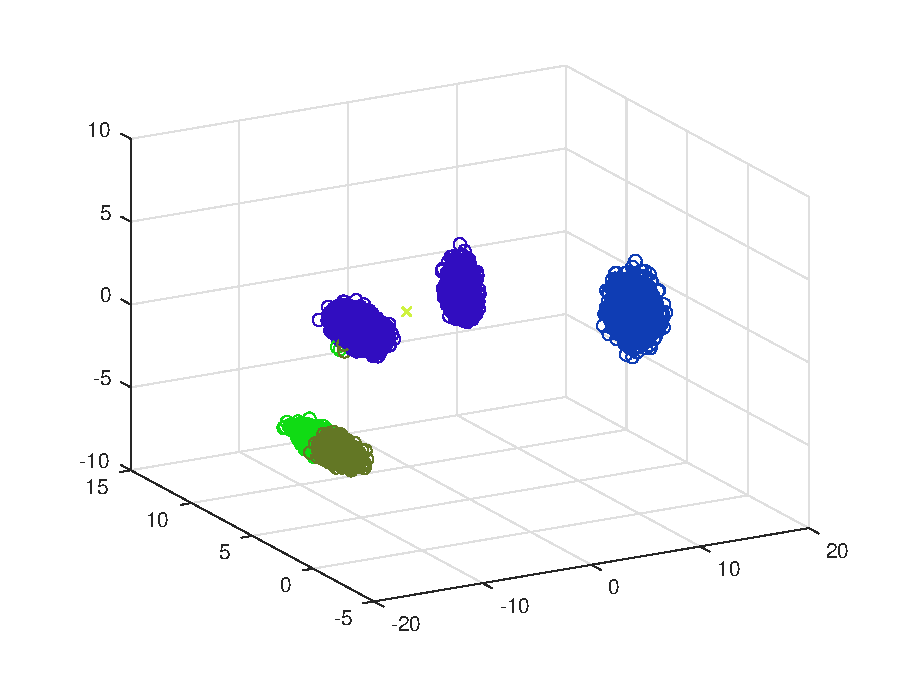
\includegraphics[width=\textwidth]{../src/fig/21_4_clusters.eps}
        \caption[]{4 \emph{clusters}}
        \label{fig:21:4c}
    \end{subfigure}
    \quad
    \begin{subfigure}[b]{0.3\textwidth}
        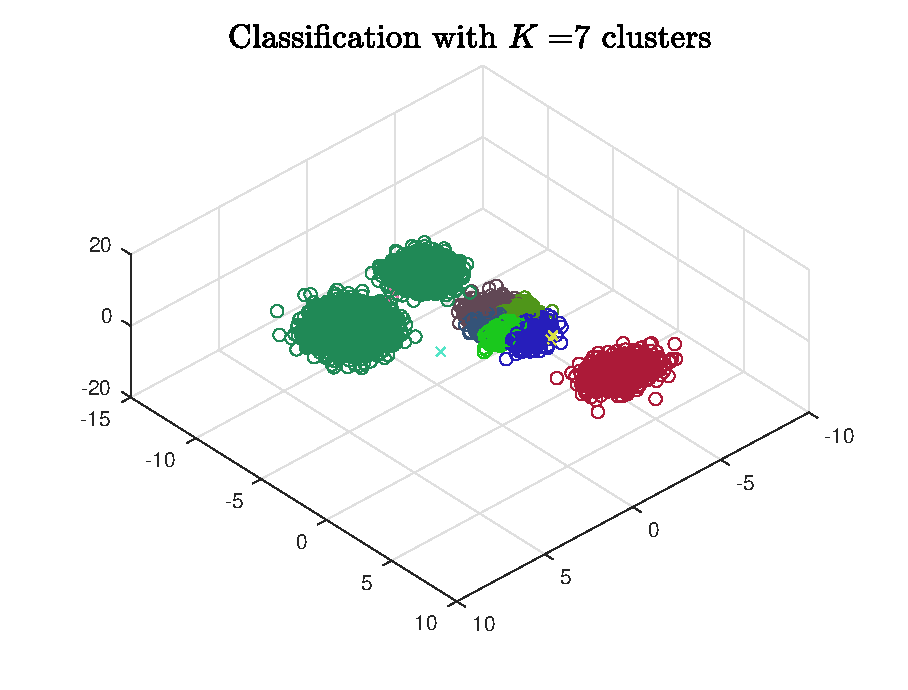
\includegraphics[width=\textwidth]{../src/fig/21_7_clusters.eps}
        \caption[]{7 \emph{clusters}}
        \label{fig:21:7c}
    \end{subfigure}
    \vskip\baselineskip
    \begin{subfigure}[b]{0.3\textwidth}
        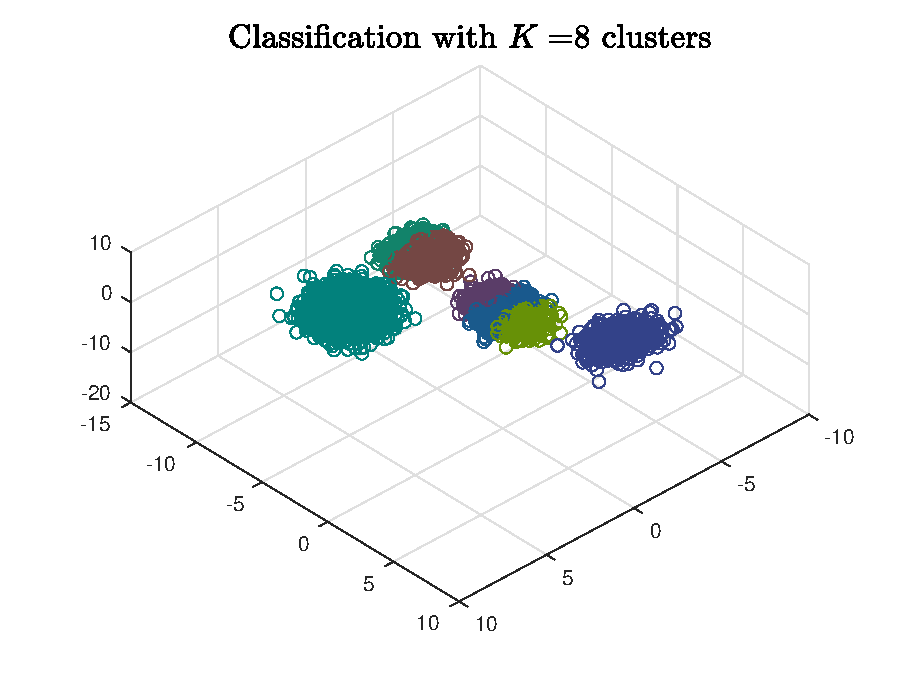
\includegraphics[width=\textwidth]{../src/fig/21_8_clusters.eps}
        \caption[]{8 \emph{clusters}}
        \label{fig:21:8c}
    \end{subfigure}
    \quad
    \begin{subfigure}[b]{0.3\textwidth}
        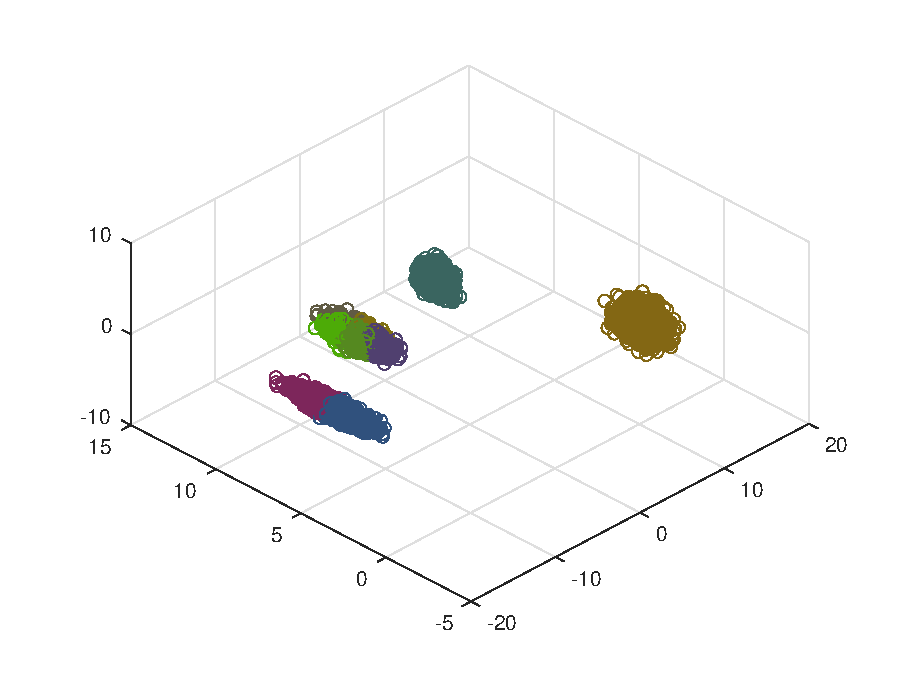
\includegraphics[width=\textwidth]{../src/fig/21_9_clusters.eps}
        \caption[]{9 \emph{clusters}}
        \label{fig:21:9c}
    \end{subfigure}
    \quad
    \begin{subfigure}[b]{0.3\textwidth}
        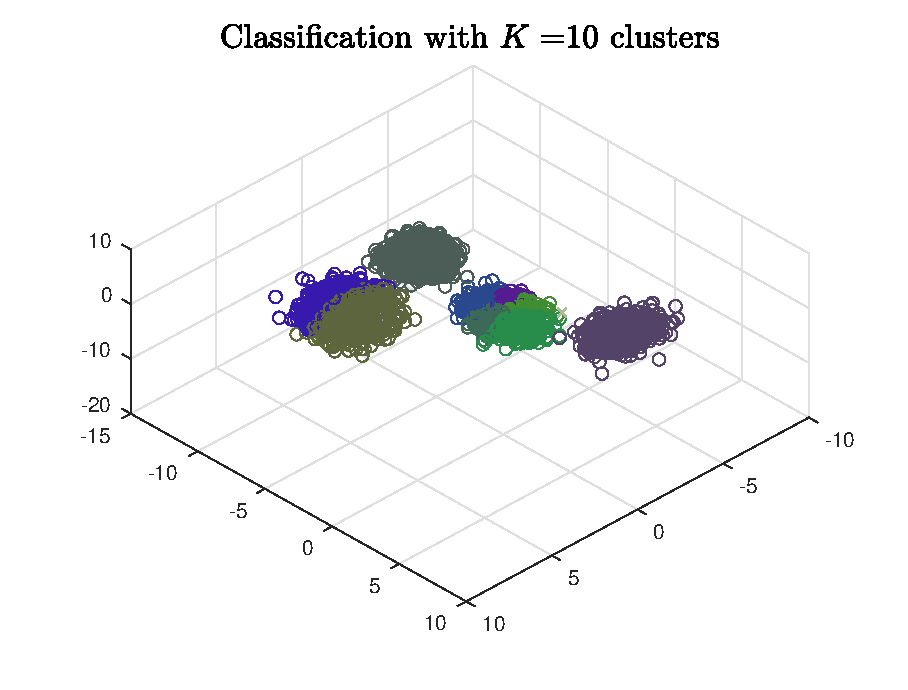
\includegraphics[width=\textwidth]{../src/fig/21_10_clusters.eps}
        \caption[]{10 \emph{clusters}}
        \label{fig:21:10c}
    \end{subfigure}
    \caption{Clasificación de la base de datos sintética}
    \label{fig:21:clusters}
\end{figure}

\begin{figure}
    \centering
    \begin{subfigure}[b]{0.3\textwidth}
        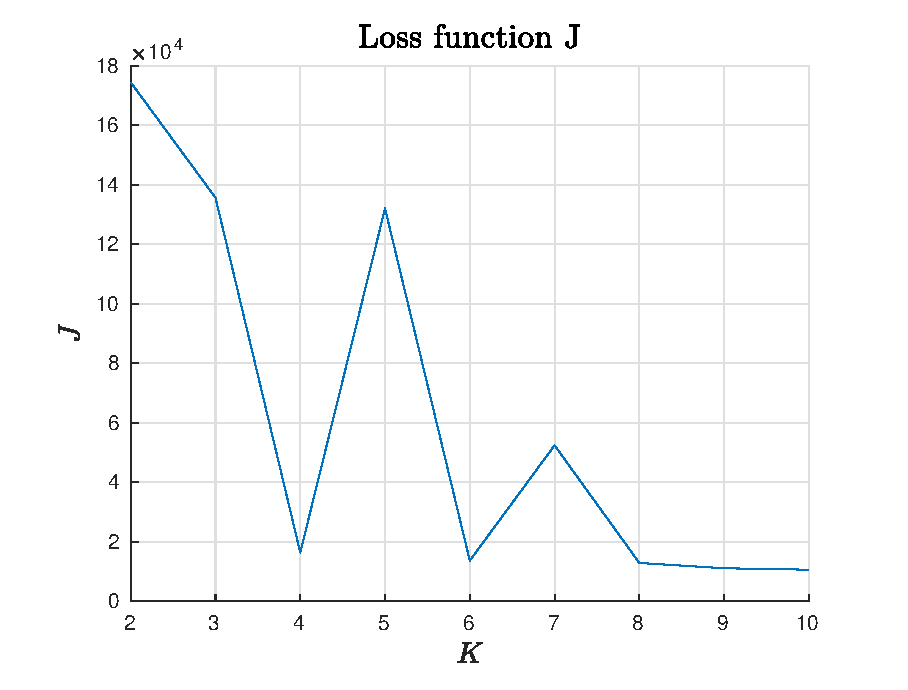
\includegraphics[width=\textwidth]{../src/fig/21_J_loss.eps}
        \caption[]{Evolución de la función de coste ($J$)}
        \label{fig:21:loss}
    \end{subfigure}
    \quad
    \begin{subfigure}[b]{0.3\textwidth}
        \includegraphics[width=\textwidth]{../src/fig/21_trace1.eps}
        \caption[]{Evolución de la métrica $Trace \left( S_T^{-1} S_W \right)$}
        \label{fig:21:trace:1}
    \end{subfigure}
    \quad
    \begin{subfigure}[b]{0.3\textwidth}
        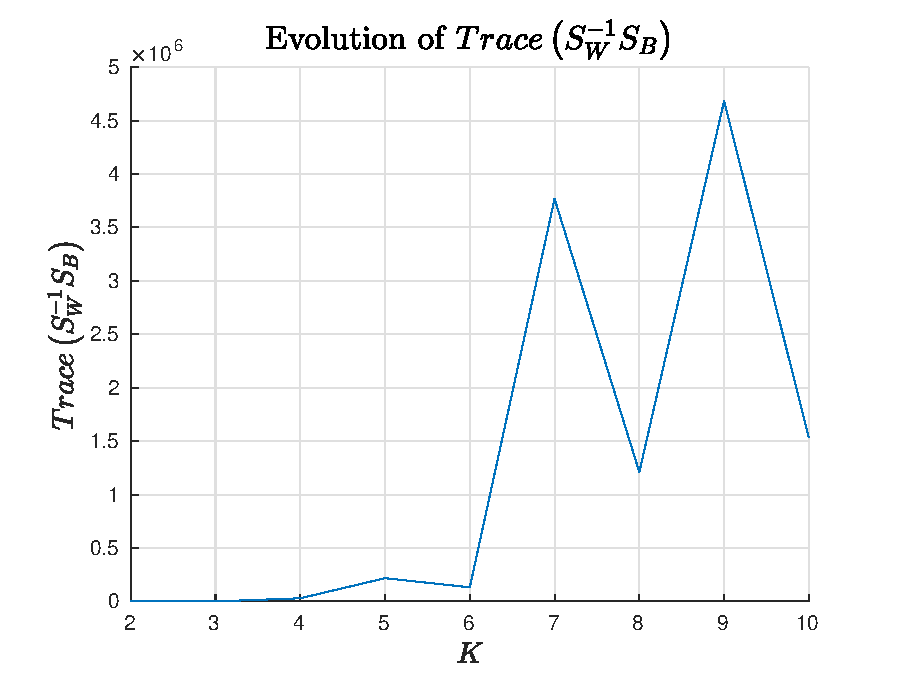
\includegraphics[width=\textwidth]{../src/fig/21_trace2.eps}
        \caption[]{Evolución de la métrica $Trace \left( S_W^{-1} S_B \right)$}
        \label{fig:21:trace:2}
    \end{subfigure}
    \caption{Evolución de las diversas métricas usadas en la clasificación}
    \label{fig:21:metrics}
\end{figure}

% Trace 2 is great, Trace 1 not good, because it decays constantly. It does so
% because as we increase the number of clusters, each of them is more compact,
% so the "within" metric improves.
%
% The J function behaves sometimes roughly like Trace 1
%
% We want to minimize Trace 1 and maximize Trace 2
%
% Trace 2 increases greatly when different clusters are classified as such,
% while Trace 1 does slightly decrease in the same situation.
%
% Because of this, Trace 2 is the best metric

Los dos cálculos de traza aportan información sobre la clasificación. Esto se
debe a que estos cálculos expresan conceptos distintos. El cálculo
$Trace \left( S_T^{-1} S_W \right)$ aporta información sobre la compactación de
los datos dentro de un \emph{cluster}, mientras que
$Trace \left( S_W^{-1} S_B \right)$ aporta información sobre la separación entre
los \emph{clusters}.

Es por ello que se en el entrenamiento se trata de minimizar uno y maximizar el
otro, respectivamente. Sin embargo, esto no implica que una disminución de
$Trace \left( S_T^{-1} S_W \right)$ vaya acompañada de un aumento en
$Trace \left( S_W^{-1} S_B \right)$. Esto se puede comprobar viendo las figuras
\ref{fig:21:trace:1} y \ref{fig:21:trace:2} para
$K= \left\lbrace 8, 9, 10 \right\rbrace $.

Hay otros detalles notables en estas métricas, tales como la caída en $J$ cuando
$K=4$. Esto se debe a que $K = L = 4$, y los clústeres están suficientemente
separados. Otro caso es el pico de $J$ en $K=7$. Esta subida del coste va
relacionada con el aumento de $Trace \left( S_T^{-1} S_W \right)$ para este
valor de $K$, aunque deseamos minimizar este cálculo. Este aumento se debe, como
se puede ver en la figura \ref{fig:21:7c}, porque la el clasificador ha
asignado la misma clase a dos \emph{clusters} distintos. Esto hace aumentar el
\emph{within-scatter} de esta clasificación, a la vez que hace que $J$ empeore.

Por tanto, concluimos que la evaluación del entrenamiento se debe realizar
teniendo en cuenta las tres métricas mencionadas: la función de coste $J$, y los
dos cálculos de traza.

%El cálculo de $Trace \left( S_W^{-1} S_B \right)$ es el que más información da
%sobre el rendimiento del clasificador. Cuando la clasificación empeora, el valor
%de éste cálculo disminuye notablemente ($K=4$ en la figura \ref{fig:21:trace:2}),
%mientras que $J$ y $Trace \left( S_T^{-1} S_W \right)$ aumentan en menor medida
%o se mantienen.

%Si se usa la menor $K$ que da mayor valor de $Trace \left( S_W^{-1} S_B \right)$,
%se consigue el número de clústeres óptimo para esa base de datos.

\clearpage

\section{Cuantificación de imágenes}

El script \textbf{\texttt{main\_2\_2}} contiene el código del ejercicio 2. En la
sección \ref{src:main:22} se puede ver su código fuente.

La recuantificación de la imagen se ha hecho con $K=7$ colores.

En las figuras \ref{fig:22:original:rgb} y \ref{fig:22:requant:rgb},
respectivamente, se puede ver el resultado de la clasificación.

\begin{figure}[h]
    \centering
    \begin{subfigure}[b]{0.435\textwidth}
        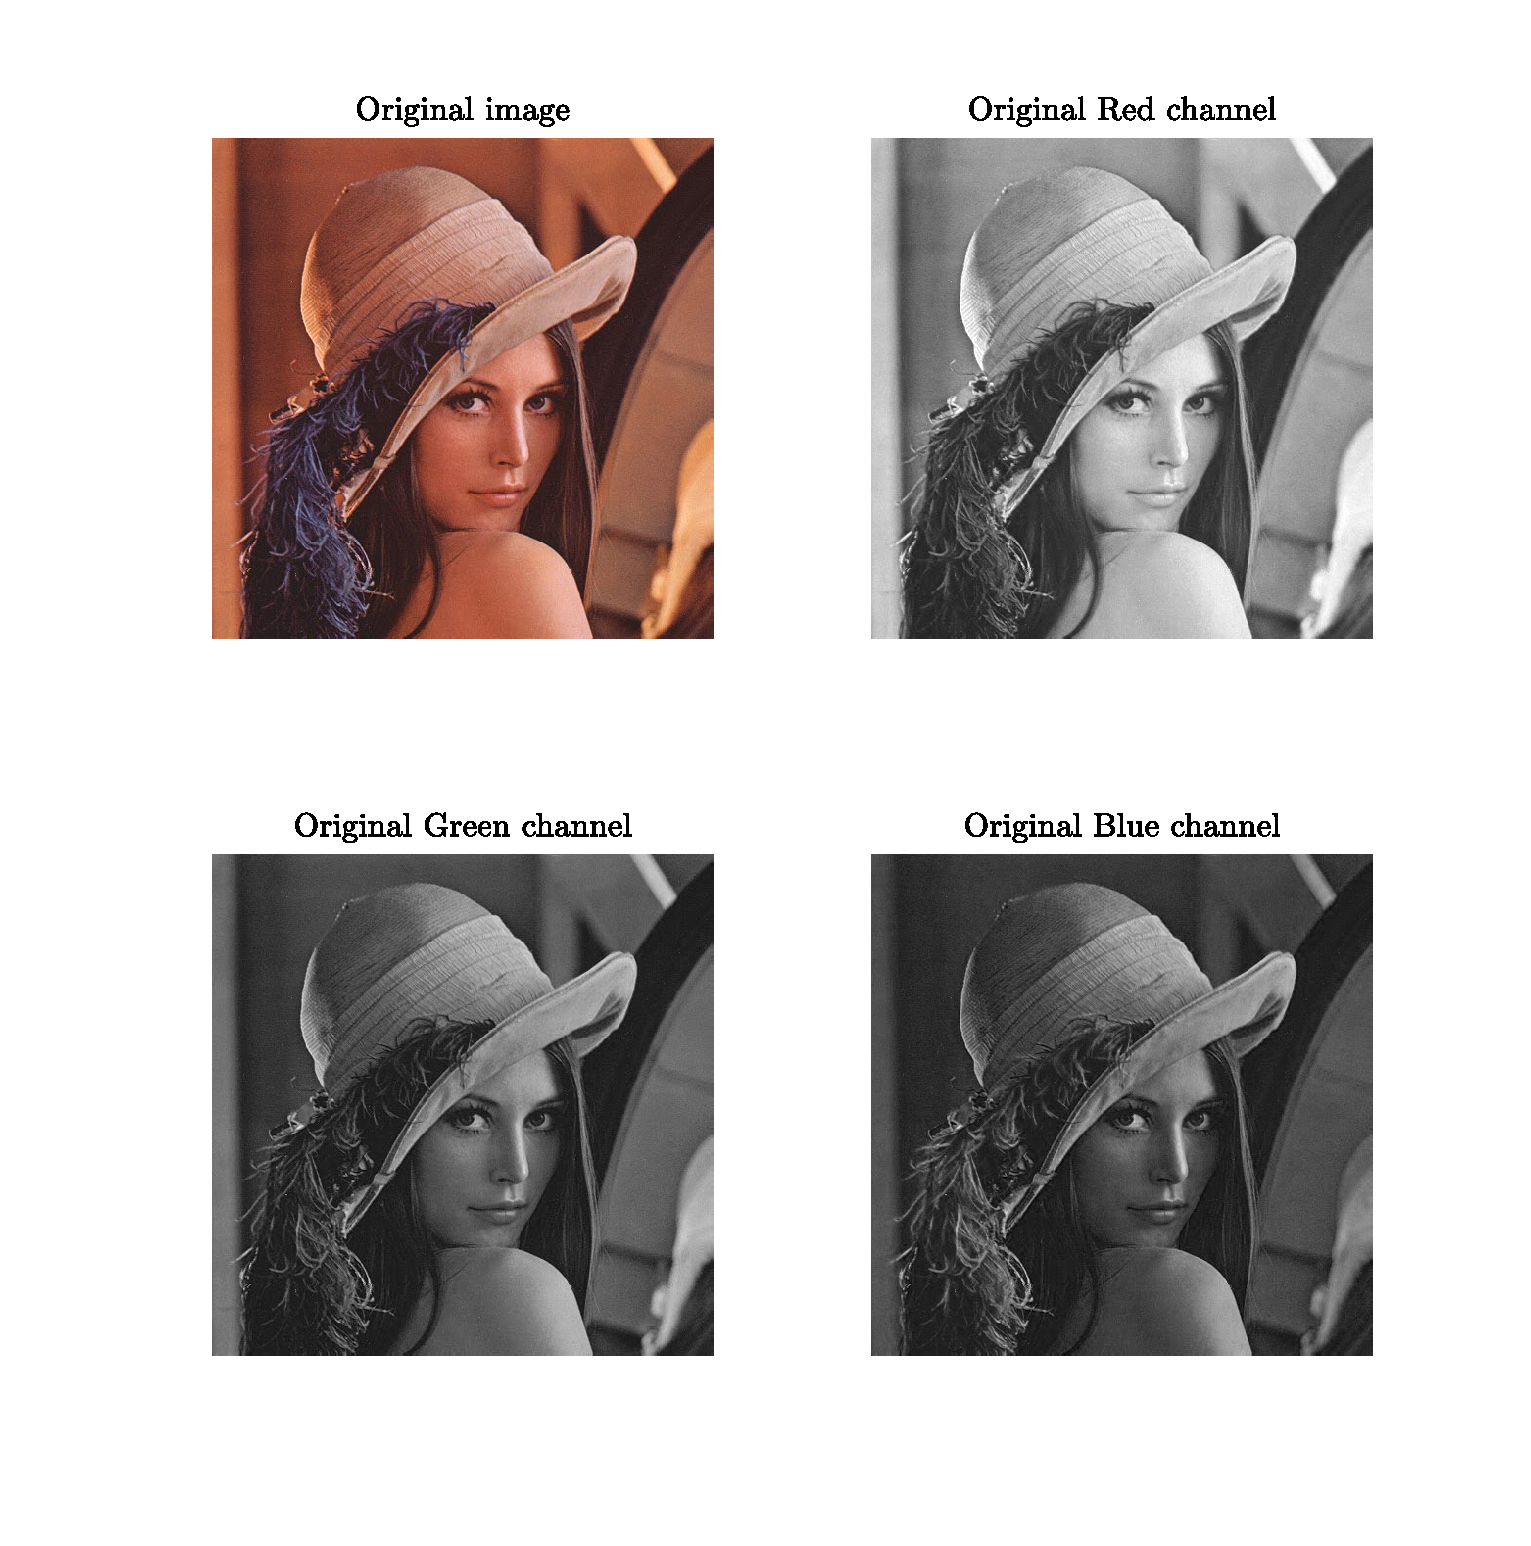
\includegraphics[width=\textwidth]{../src/fig/22_original_lena.eps}
        \caption[]{Canales de la imagen original}
        \label{fig:22:original:rgb}
    \end{subfigure}
    \quad
    %\vskip\baselineskip
    \begin{subfigure}[b]{0.435\textwidth}
        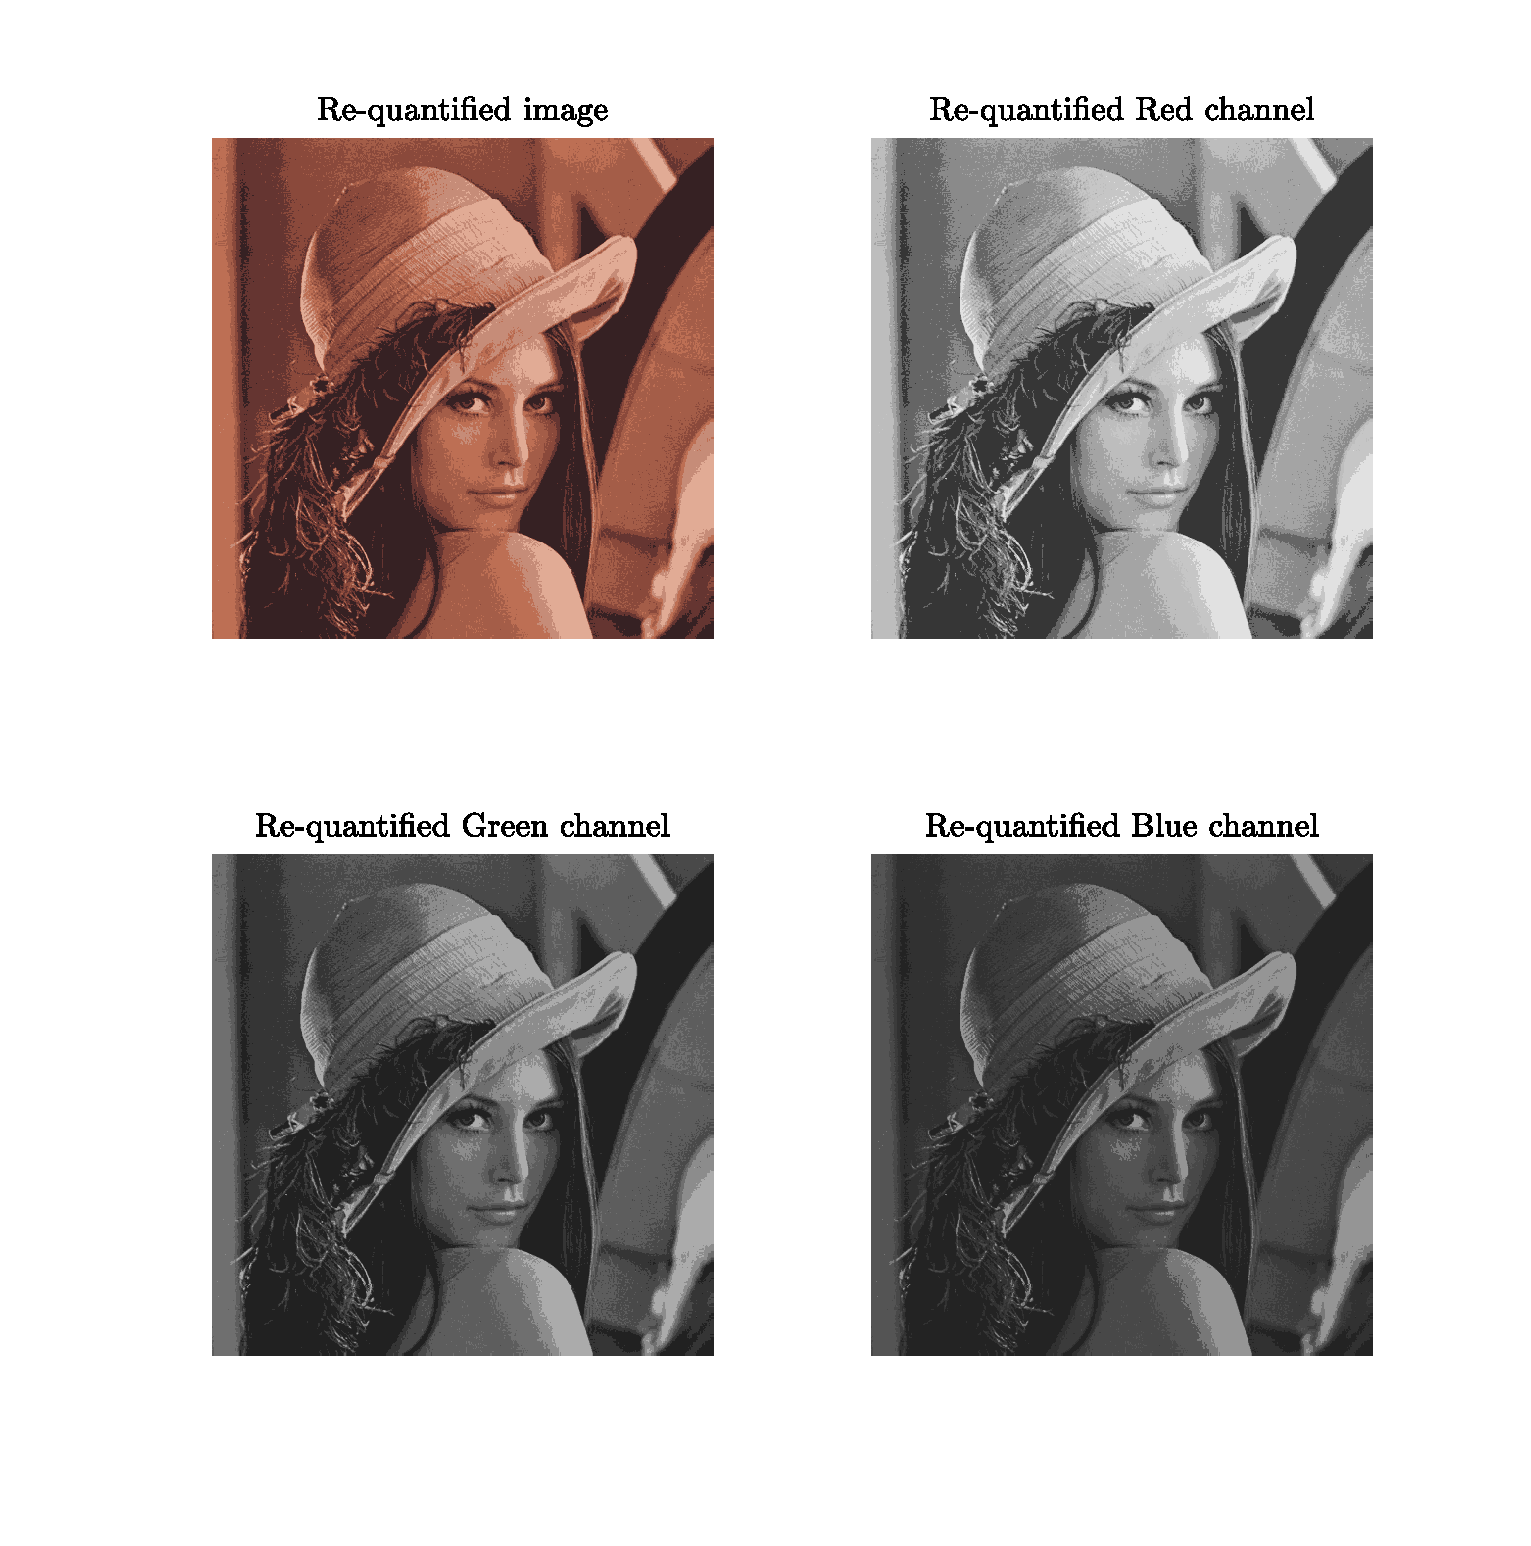
\includegraphics[width=\textwidth]{../src/fig/22_requantified_lena.eps}
        \caption[]{Canales de la imagen recuantificada}
        \label{fig:22:requant:rgb}
    \end{subfigure}
    %\quad
    \caption{Recuantificación de la imagen \emph{Lena} con $K=7$ colores}
    \label{fig:22:classification}
\end{figure}

En la figura \ref{fig:22:clusters} se pueden ver los \emph{clusters} de la
image original y de su versión recuantificada.

\begin{figure}[h]
    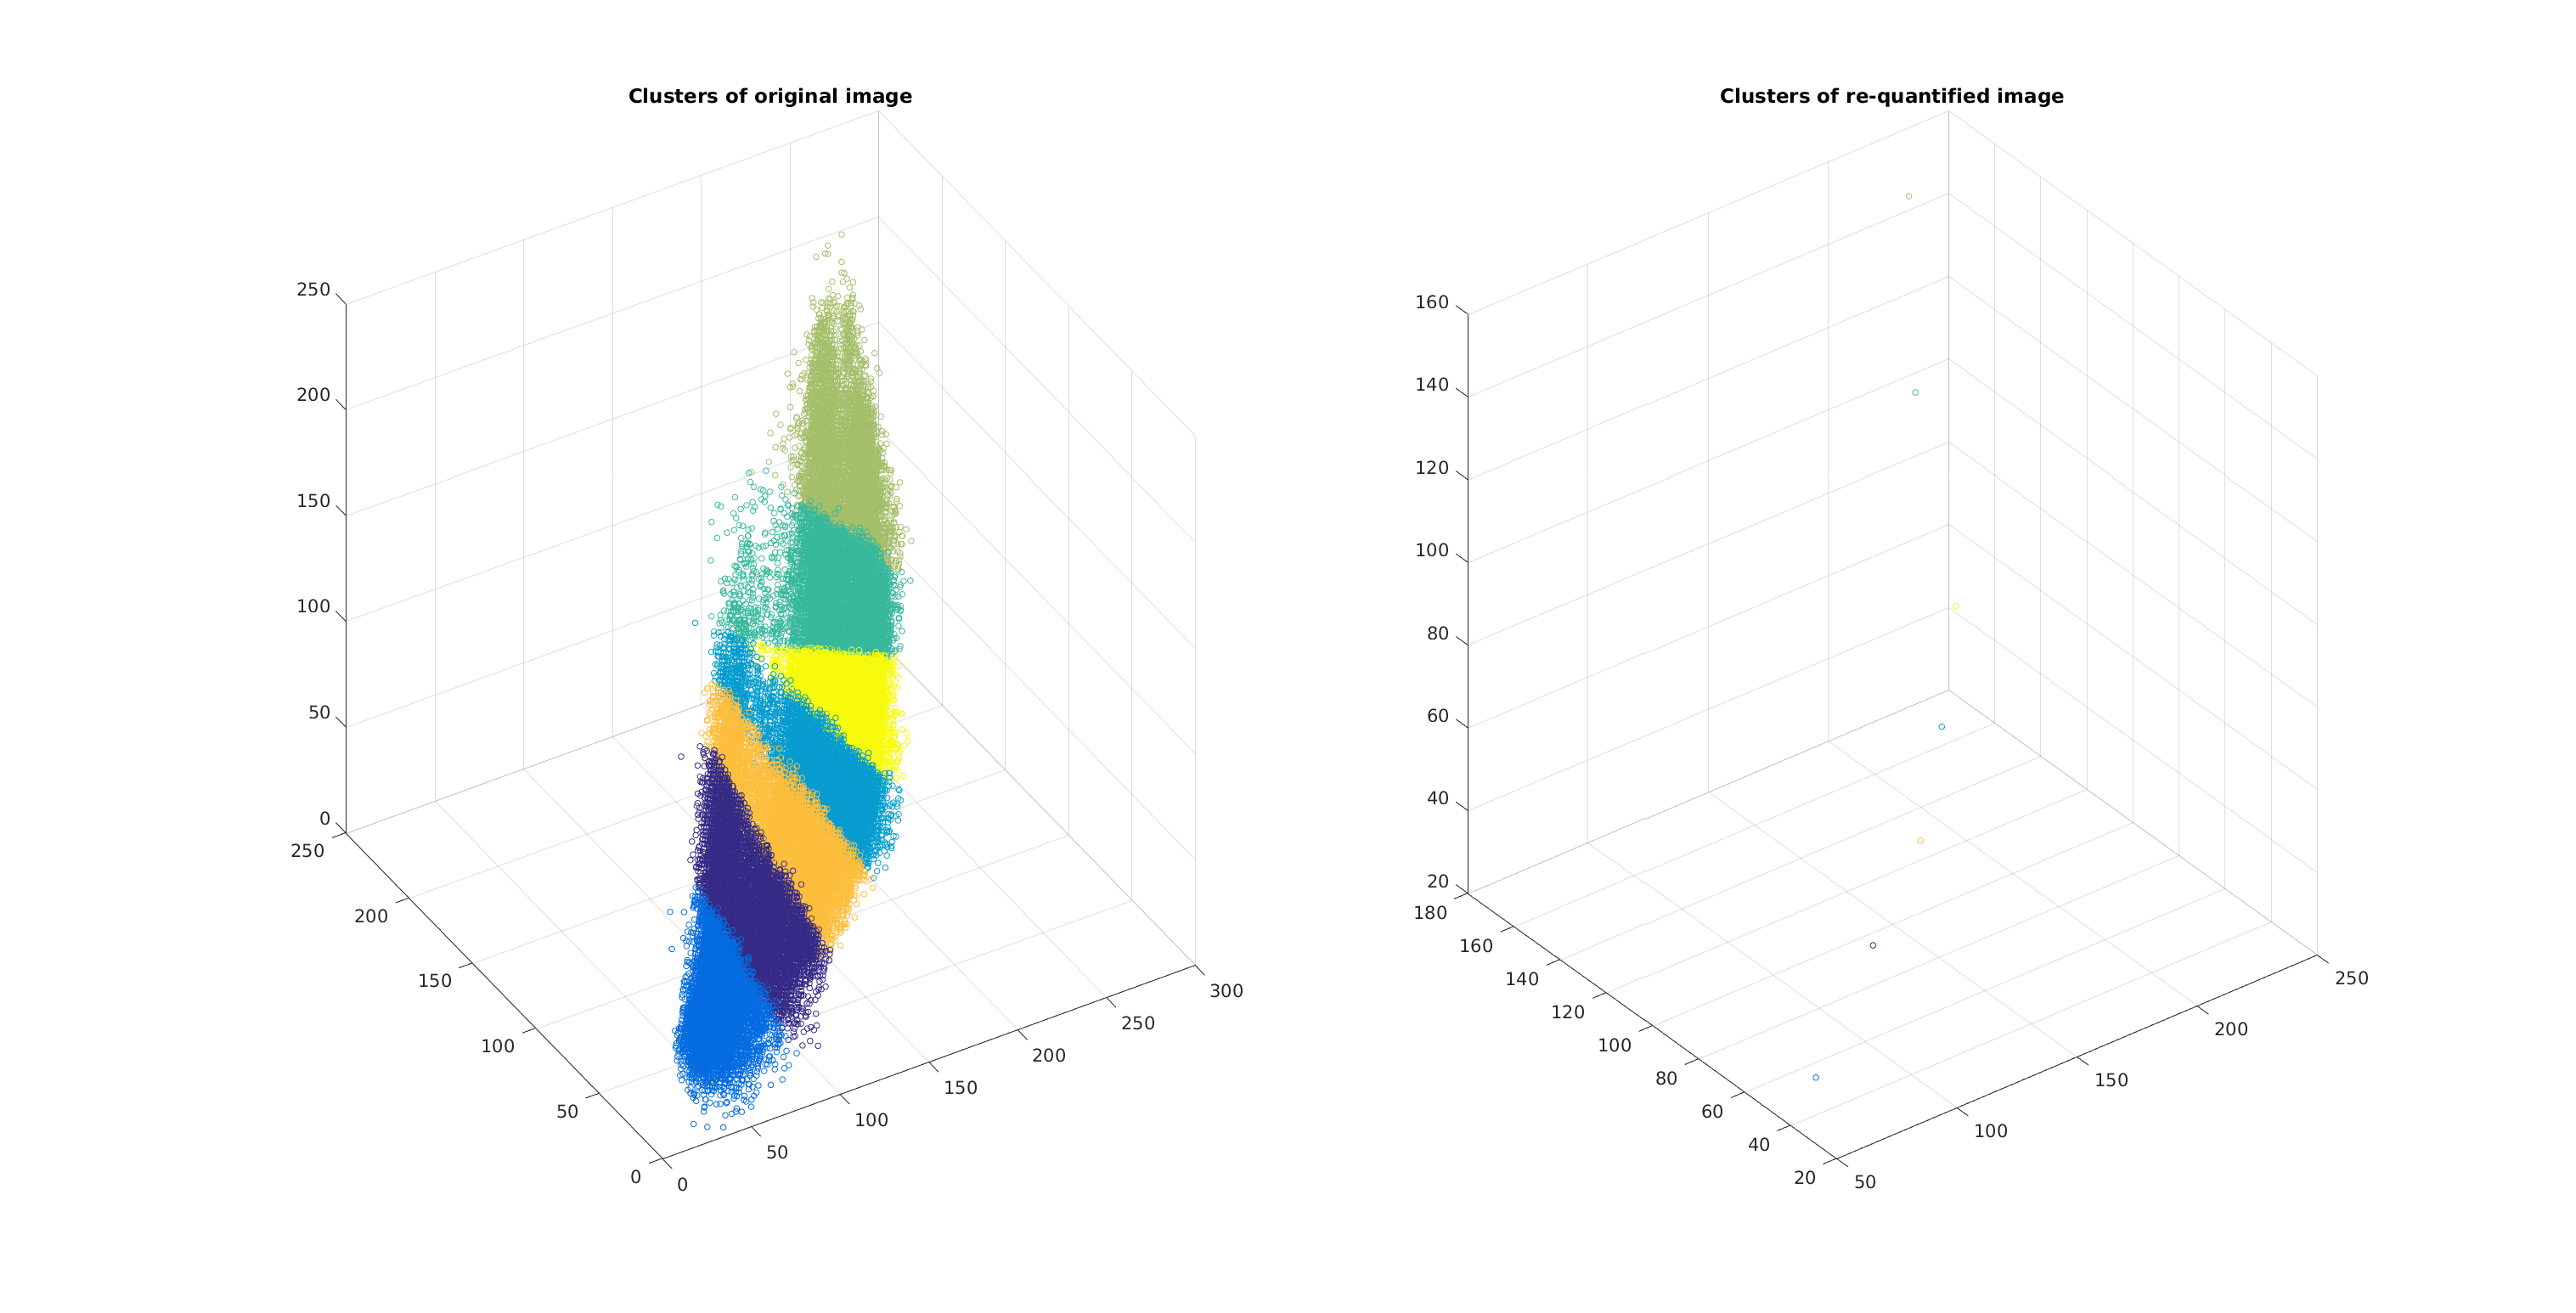
\includegraphics[width=\textwidth, height=6cm]{../src/fig/22_lena_clusters.eps}
    \caption[]{\emph{Clusters} de la imagen original y recuantificada}
    \label{fig:22:clusters}
\end{figure}

\clearpage
\newgeometry{bottom=5cm}

La evolución de los valores de la función de coste $J$ se muestra en la figura
\ref{fig:22:cost}.

\begin{figure}[h]
    \centering
    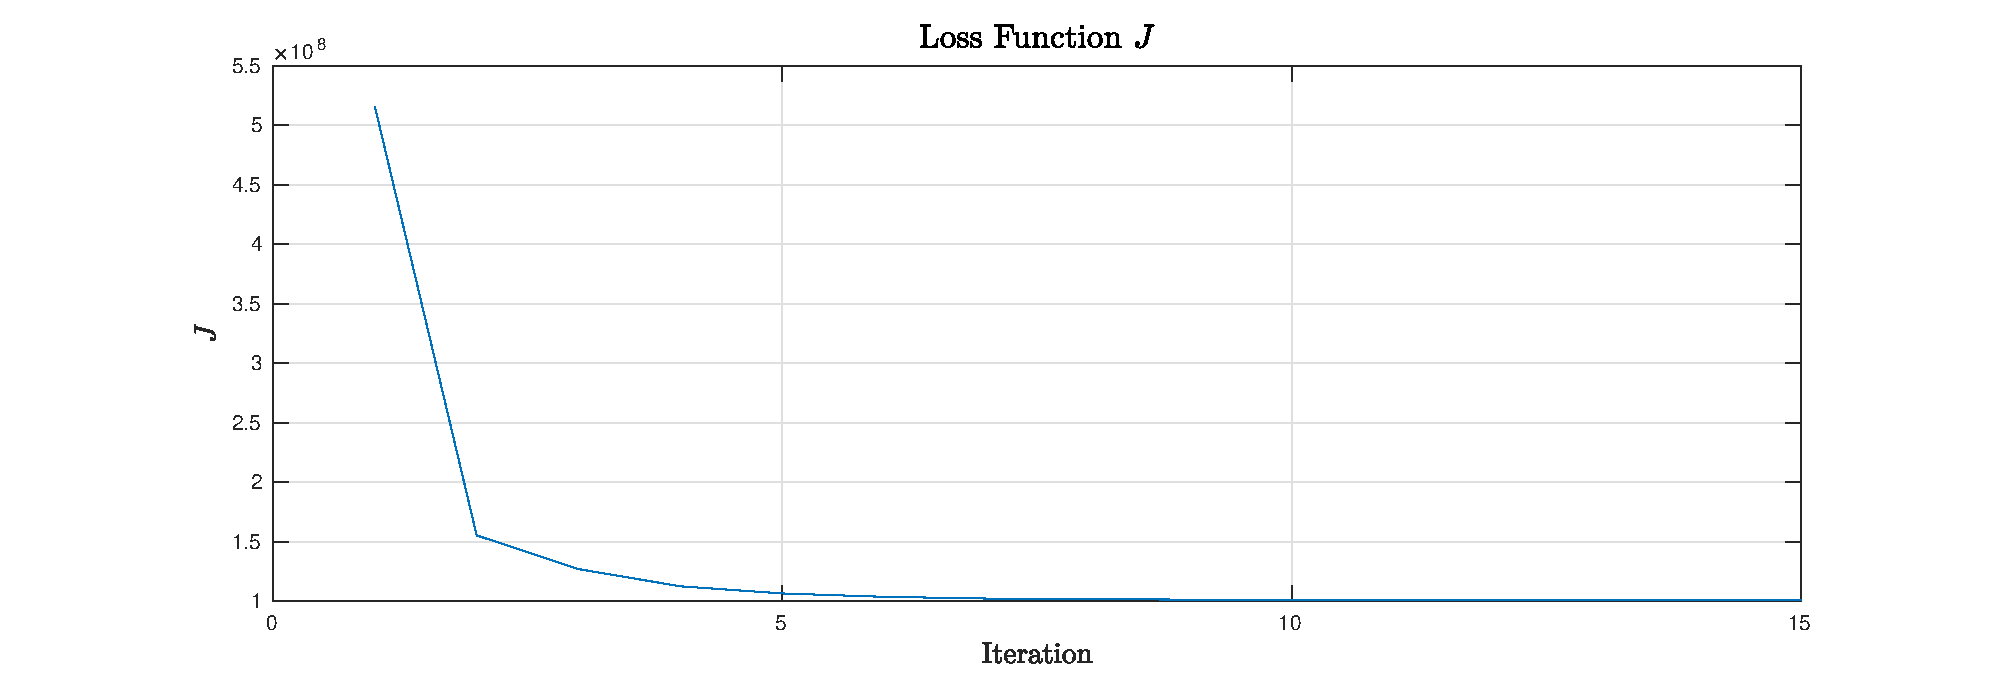
\includegraphics[width=0.7\textwidth]{../src/fig/22_cost.eps}
    \caption[]{Evolución de los valores de la función de coste $J$}.
    \label{fig:22:cost}
\end{figure}

En la figura se puede ver como el valor de la función desciende rápidamente, de
manera que a partir de la iteración 6, la clasificación prácticamente no varia.
Las iteraciones siguientes se han calculado para cumplir con la condición del
clasificador, que dicta que se continue iterando hasta
que $\Delta J \leq th = 0.0005$.

La evolución de los valores de $Trace \left( S_T^{-1} S_W \right)$ y
$Trace \left( S_W^{-1} S_B \right)$ se muestra en la figura \ref{fig:22:traces}.

\begin{figure}[h]
    \centering
    \begin{subfigure}[b]{0.435\textwidth}
        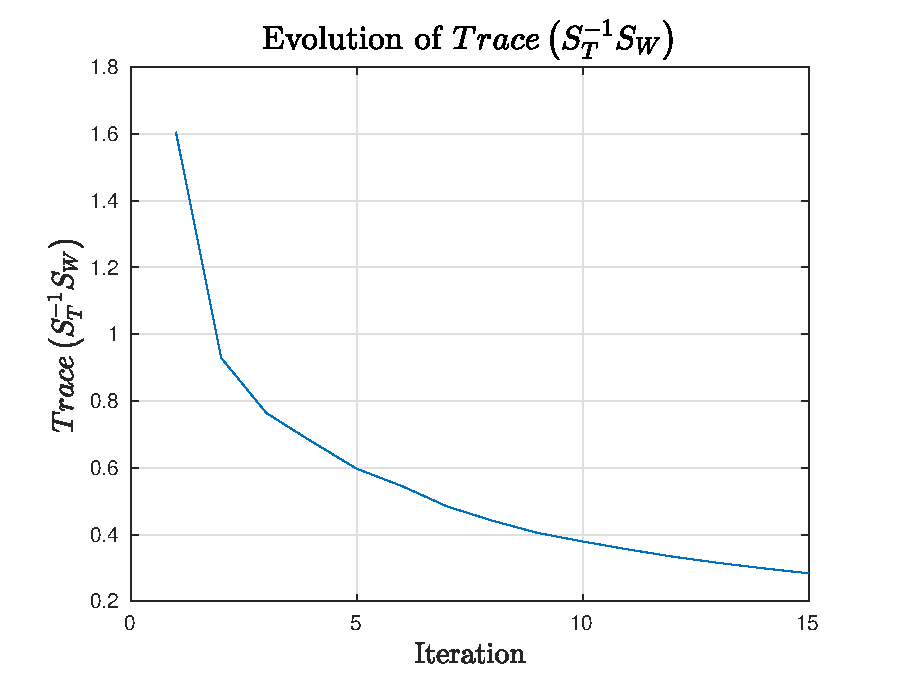
\includegraphics[width=\textwidth]{../src/fig/22_trace1.eps}
        \caption[]{Evolución de $Trace \left( S_T^{-1} S_W \right)$}
        \label{fig:22:trace:1}
    \end{subfigure}
    \quad
    %\vskip\baselineskip
    \begin{subfigure}[b]{0.435\textwidth}
        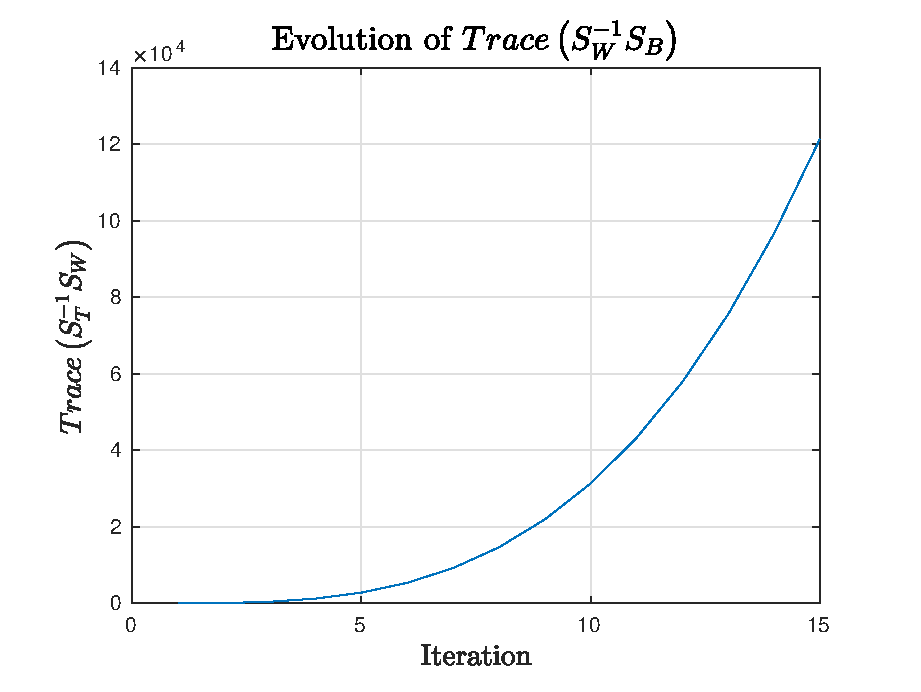
\includegraphics[width=\textwidth]{../src/fig/22_trace2.eps}
        \caption[]{Evolución de $Trace \left( S_W^{-1} S_B \right)$}
        \label{fig:22:trace:2}
    \end{subfigure}
    %\quad
    \caption{Evolución de las métricas de Traza según cada interación del
    clasificador \emph{K-Means}}
    \label{fig:22:traces}
\end{figure}

Estos valores concuerdan con la optimización de la clasificación; tenemos un
valor que disminuye, para $Trace \left( S_T^{-1} S_W \right)$, y un valor que
incrementa, para $Trace \left( S_W^{-1} S_B \right)$.

Como se muestra en \cite{zanibbi_clustering_2010} (página 22) las expresiones de
los cálculos de traza corresponden a las ecuaciones \eqref{eq:trace:2} y
\eqref{eq:trace:1}, donde $\lambda_i$ representa el valor propio de la matriz
\emph{''within-cluster scatter''} ($S_W$).

\begin{align}
    \label{eq:trace:2}
    trace \left[ S_W^{-1} S_B \right] &= \sum_{i=1}^{d} \lambda_i \\
    \label{eq:trace:1}
    trace \left[ S_T^{-1} S_B \right] &= \sum_{i=1}^{d} \frac{1}{1 + \lambda_i}
\end{align}

Siendo así, la evolución de los valores de estas métricas corresponde a una
disminución de los mencionados autovalores.

\bigskip

El cálculo de los bits necesarios para almacenar las imágenes sigue la siguiente
ecuación:

\begin{equation} \label{eq:bits}
    N_{bits} = \lceil log_2 \left( K \right) \rceil \cdot N_{p_{img}} \cdot N_{channels}
\end{equation}

donde $N_{p_{img}}$ es el número de píxeles en la imagen y $N_{channels}$, el
número de canales de color (en el caso RGB son 3).

\bigskip

El resultado del cálculo se muestra a continuación:

\begin{verbatim}
>> main_2_2
We need 6291456 bits to store the Lena image
We need 3145728 bits to store the quantified image
\end{verbatim}

Con los centroides obtenidos de la imagen \emph{Lena} con $K=7$, se ha
cuantificado una imagen del guitarrista Paco de Lucía. Los resultados se
muestran en la figura \ref{fig:22:paco}.

Los resultados de aplicar los centroides calculados en una imagen aplicados a
otra de diferente varian dependiendo de la imagen con la que se han calculado.
En nuestro caso, la imagen \emph{Lena} posee una gama cromática reducida. Eso
hace que los centroides escogidos sean bastante parecidos. Por eso, colores como
el marrón se representan muy bien en la imagen \emph{Paco} (bastante parecido al
color general de \emph{Lena}) pero en cambio, el blanco se convierte en marrón.

Un posible uso de esta técnica seria la compresión de imágenes, vía una tabla de
colores. Si se obtuviera un gran número de centroides (ej: 256) con una imagen
de gran variabilidad cromática, se podría re-cuantificar otras imágenes con
estos centroides, y el resultado seria fiable, ya que la mayoría de posibles
colores estarían representados por los centroides.

Otro posible uso serviría para fines artísticos, ya que el efecto de sustituir
los colores de una imagen por los de otra puede ser atractivo para el público.

\begin{figure}[h]
    \centering
    \begin{subfigure}[b]{0.48\textwidth}
        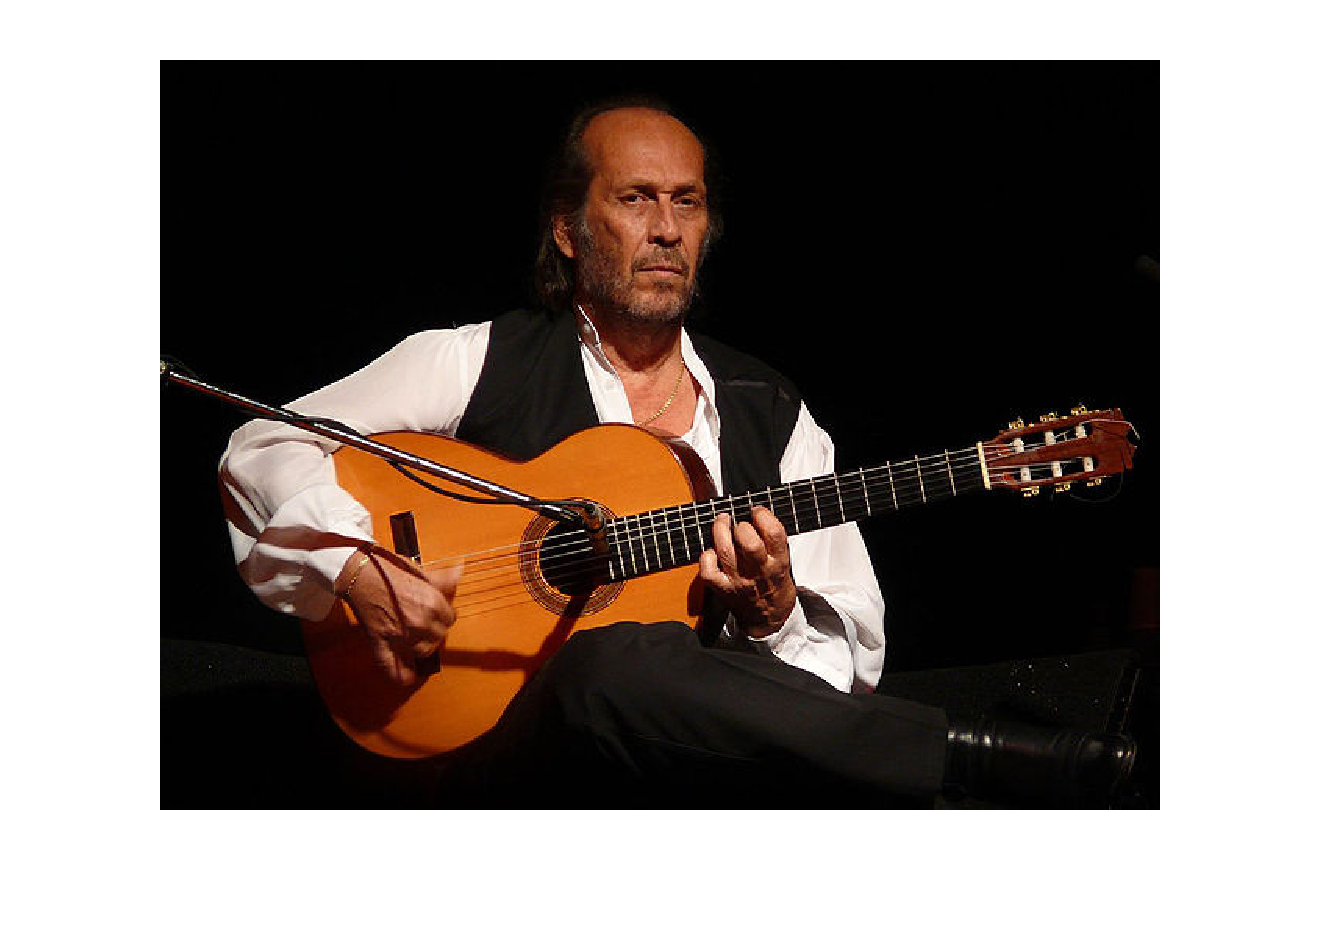
\includegraphics[width=\textwidth]{../src/fig/22_paco_original.eps}
        \caption[]{Imagen original}
        \label{fig:22:paco:original}
    \end{subfigure}
    \quad
    %\vskip\baselineskip
    \begin{subfigure}[b]{0.48\textwidth}
        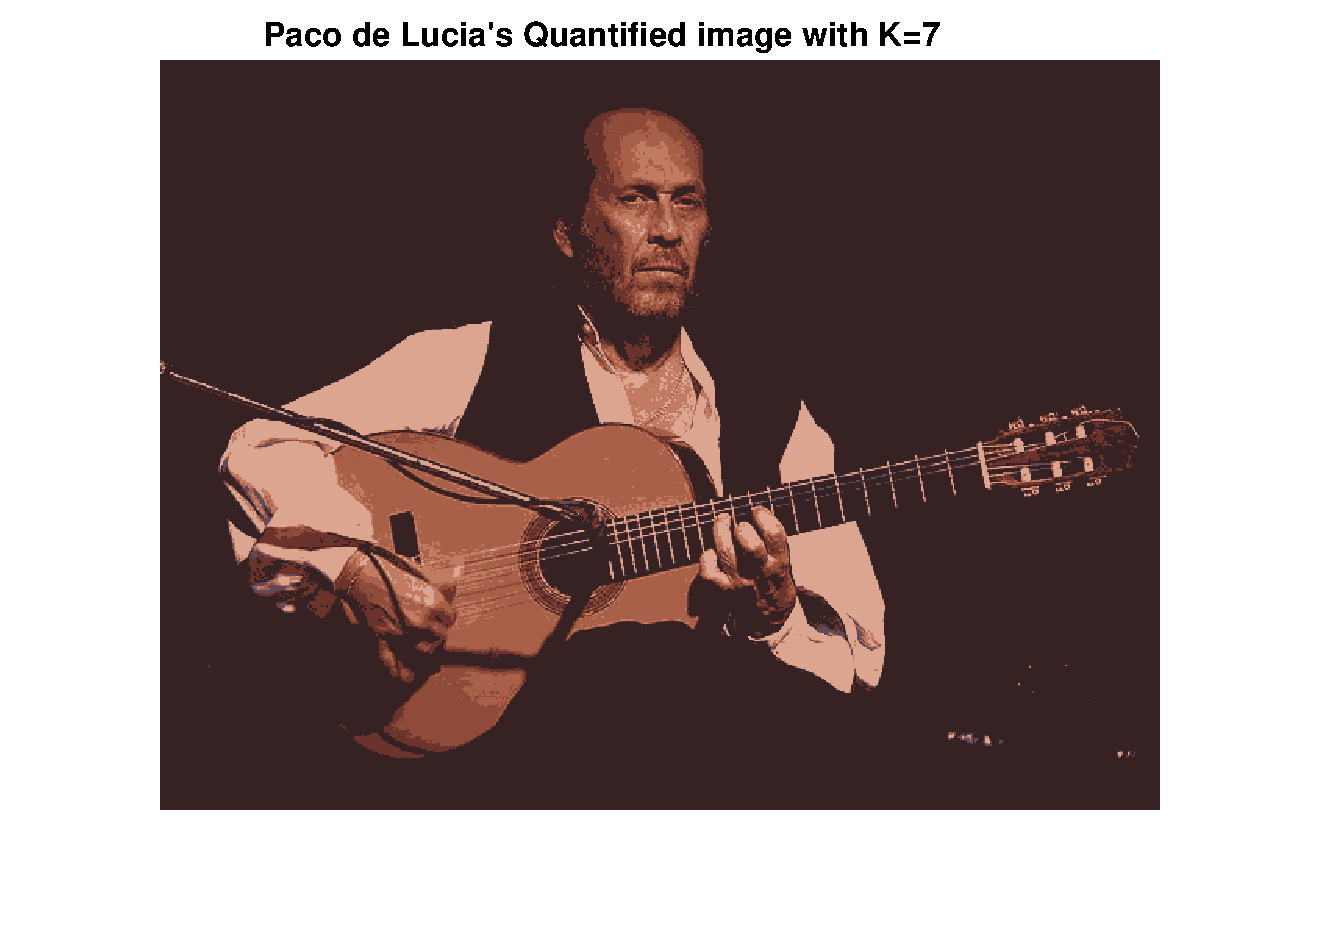
\includegraphics[width=\textwidth]{../src/fig/22_paco_requant.eps}
        \caption[]{Imagen recuantificada}
        \label{fig:22:paco:requant}
    \end{subfigure}
    %\quad
    \caption{Recuantificación de la imagen \emph{Paco} con los centroides
             obtenidos con la imagen \emph{Lena}}
    \label{fig:22:paco}
\end{figure}

\clearpage
\restoregeometry

\section{Identificación de clústeres en una base de datos propia}

El script \textbf{\texttt{main\_2\_3}} contiene el código del ejercicio 3. En
la sección \ref{src:main:23} se puede ver su código fuente.

Para este ejercicio se ha usado la base de datos \textbf{Iris Plants Database}
(\url{http://archive.ics.uci.edu/ml/datasets/Iris}). Esta base de
datos contiene información de la longitud y anchura de los sépalos y pétalos de
varias espécies de flores del género \emph{Iris}.

En la descripción de la base de datos se especifica que los 150 vectores están
distribuidos en 3 clases. Una de ellas es linealmente separable de las otras
dos, mientras que las otras dos restantes, \emph{NO} son linealmente separables.

En la figura \ref{fig:23:scatter} se pueden ver los \emph{clusters}
clasificados. Claramente se muestra una clase separada de las otras dos.

\begin{figure}[h]
    \centering
    \begin{subfigure}[b]{0.435\textwidth}
        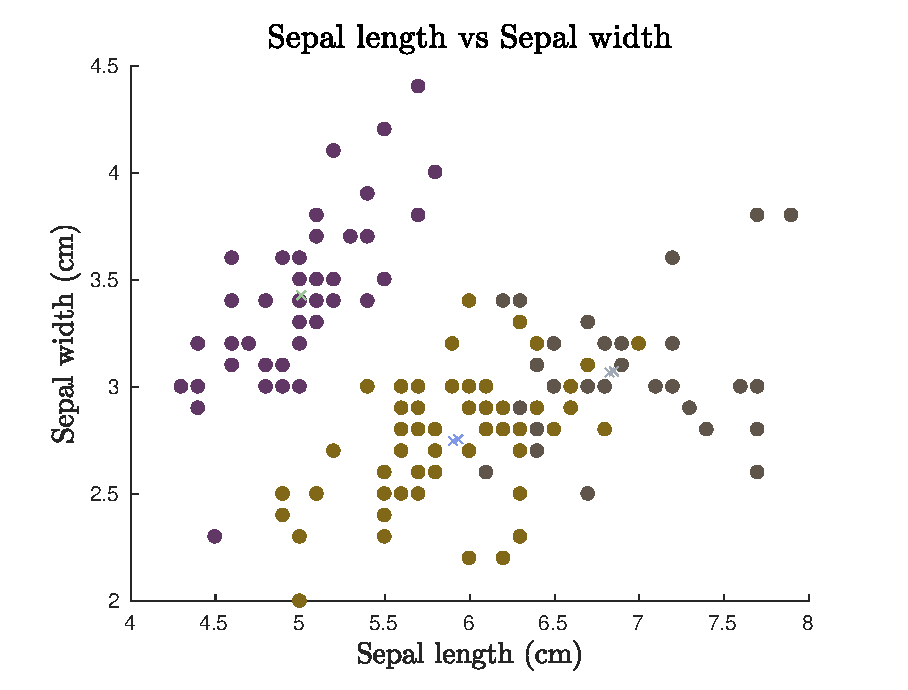
\includegraphics[width=\textwidth]{../src/fig/23_sepal.eps}
        \caption[]{\emph{Clusters} de las características de los sépalos}
        \label{fig:23:scatter:sepals}
    \end{subfigure}
    \quad
    %\vskip\baselineskip
    \begin{subfigure}[b]{0.435\textwidth}
        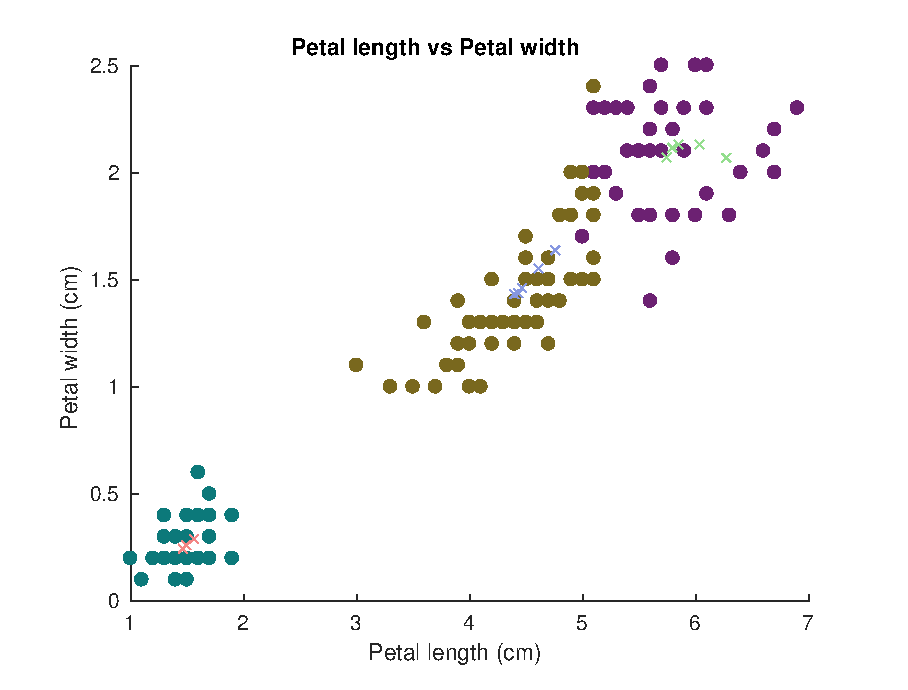
\includegraphics[width=\textwidth]{../src/fig/23_petal.eps}
        \caption[]{\emph{Clusters} de las características de los pétalos}
        \label{fig:23:scatter:petals}
    \end{subfigure}
    %\quad
    \caption{Resultado de la clasificación de la base de datos
             \textbf{Iris Plants Database}}
     \label{fig:23:scatter}
\end{figure}

Para evaluar el rendimiento del clasificador, como esta base de datos es
etiquetada, podemos comprobar el índice de aciertos. Sin embargo, esto no es una
tarea simple.

El problema radica en que los centroides del clasificador se asignan
aleatoriamente. Esto hace que no podamos saber qué especie de \emph{Iris}
corresponde a cada centroide. Por tanto, no podemos medir cuántos vectores han
sido clasificados correctamente comparando las etiquetas.

Para poder evaluar el rendimiento del clasificador, hemos aplicado un producto
matricial sobre el vector de etiquetas resultante de la clasificación, y lo
hemos representado con un código de colores. La figura \ref{fig:23:heatmap} muestra esta
representación.

Esta forma de mostrar las etiquetas permite una evaluación visual aproximada de
cuán bien trabaja el clasificador. La lógica tras esta representación es:

\begin{itemize}
    \item Si todas las etiquetas se detectan correctamente, la figura resultante
        mostrará 9 ($3^2$) rectángulos de distintos colores, segun el código elegido.
    \item Si hay vectores mal clasificados, éstos se mostrarán en el gráfico en
        forma de líneas de distinto color al del rectángulo en el que deberian
        pertenecer.
\end{itemize}

Esta forma de evaluar la clasificación funciona porque en la base de datos, los
vectores están ordenados de tal manera que los vectores de una misma clase
ocupan posiciones correlativas.

En la figura \ref{fig:23:heatmap:db} se muestran las etiquetas de la base de
datos. Este gráfico muestra los 9 rectángulos perfectos. En la figura
\ref{fig:23:heatmap:kmeans} se muestran las etiquetas de la clasificación. Como
indicábamos anteriormente, hay líneas de distinto color al rectángulo que las
rodea, indicando vectores mal clasificados.

El rectángulo de la parte superior izquierda de la figura representa la clase
linealmente separable de las otras dos, ya que solo muestra un solo vector mal
clasificado.

Los colores no se corresponden entre los dos gráficos, debido a la asignación
aleatoria de los centroides mencionada anteriormente.

\begin{figure}[h]
    \centering
    \begin{subfigure}[b]{0.435\textwidth}
        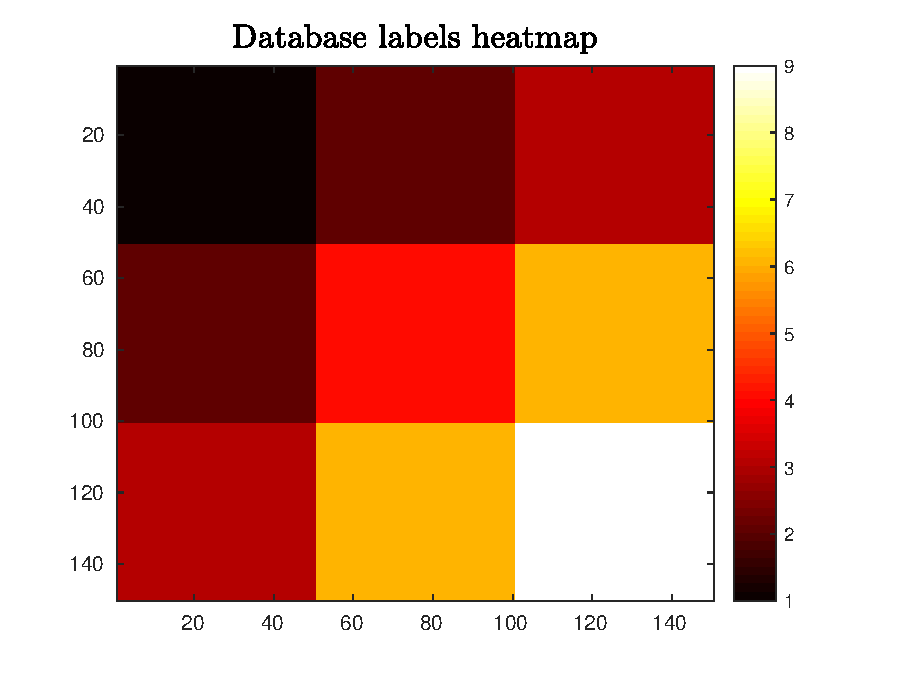
\includegraphics[width=\textwidth]{../src/fig/23_db_heatmap.eps}
        \caption[]{Etiquetas de la base de datos}
        \label{fig:23:heatmap:db}
    \end{subfigure}
    \quad
    %\vskip\baselineskip
    \begin{subfigure}[b]{0.435\textwidth}
        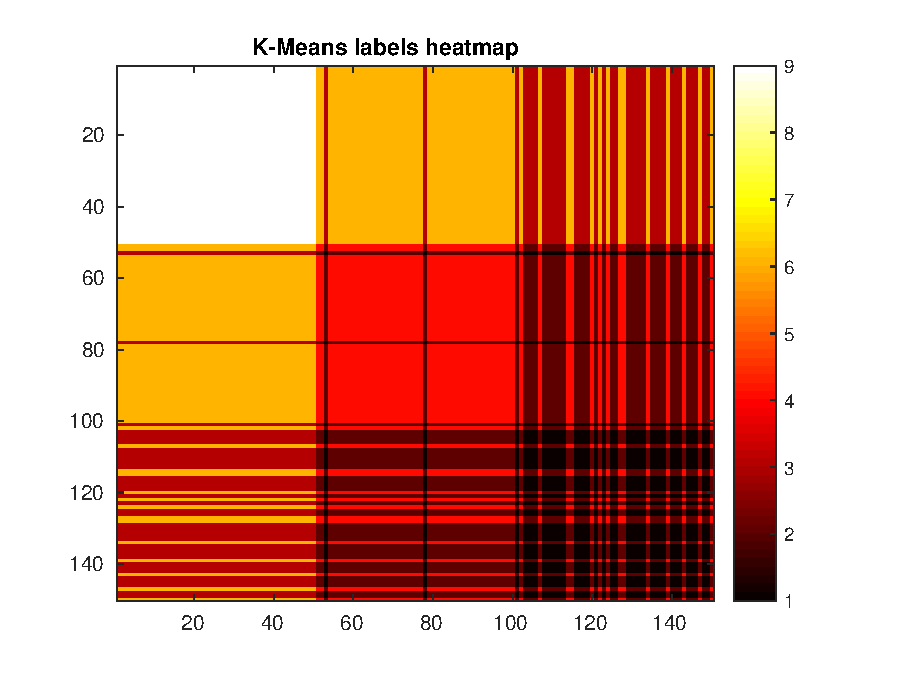
\includegraphics[width=\textwidth]{../src/fig/23_kmeans_heatmap.eps}
        \caption[]{Etiquetas resultado de la clasificación}
        \label{fig:23:heatmap:kmeans}
    \end{subfigure}
    %\quad
    \caption{Representación de las etiquetas de la base de datos y de la
        clasificación.}
     \label{fig:23:heatmap}
\end{figure}

\clearpage

\section{Código fuente}
\label{sec:src_code}

A continuación se encuentra el código fuente generado para la resolución de
este laboratorio

\subsection{\texttt{main\_2\_1}}
\label{src:main:21}

\lstinputlisting{../src/main_2_1.m}

\subsection{\texttt{main\_2\_2}}
\label{src:main:22}

\lstinputlisting{../src/main_2_2.m}

\clearpage

\subsection{\texttt{main\_2\_3}}
\label{src:main:23}

\lstinputlisting{../src/main_2_3.m}

\clearpage

\subsection{\texttt{CLP\_Generate}}
\label{src:fun:generate}

\lstinputlisting{../src/CLP_Generate.m}

\clearpage

\subsection{\texttt{CLP\_Kmeans}}
\label{src:fun:kmeans}

\lstinputlisting{../src/CLP_Kmeans.m}

\clearpage

\bibliographystyle{plain}
\bibliography{bibliography.bib}

\end{document}
